\documentclass[a4paper, 12pt, final]{article}

\usepackage[utf8]{inputenc}
\usepackage[francais]{babel}
\usepackage[french]{varioref}
\usepackage{layout} 
\usepackage{listings} 
\usepackage[comma,authoryear]{natbib}
\usepackage{graphicx}

\title{ ELE 470 - Tab Bars and Pickers }

\author{ Laïla Atrmouh }

\date{Tuesday 23 October 2012}

\begin{document}

\maketitle  
   
\rule[0.5ex]{\textwidth}{0.1mm}
\section{Introduction}
The purpose of this lab is to see how we can set up tab bars and pickers. These two types of objects have a very specific role. Generally, the tab bar is used to show the different functionalities of the application; for example in the Clock Application of the iPhone, there is a tab bar with different tab bar items linked to each functionality: world clock, alarm, chronometer, .. It is different for the picker which is used to offer a choice to the user. A picker can be used inside of a tab bar view; for example in the clock view, a picker is used to fix at what time shall the alarm be setted.

\section{Methods}
The tab bars are not complicated to use: you need to do a xib file for each tab bar item you have in the tab bar, and then make connections between the several views using the Interface Builder interface (by connecting the views to the File's Owner). \\
The picker is more complicated to use: you have to implement the method pickerView and again, the semantic of the Objective-C language is very particular. We also saw how to use sounds in an app: a special library called AudioToolbox must be used by importing the head file, but also by configuring the build path. Indeed, the library needs to be linked in order that the compiler "knows" that we are using a library.

\section{Conclusion}
The tab bars are really useful for apps who have a lot of functionalities. This lab enable us to use different items proposed by the object library. We will definitely use these objects for our personnal projects.

\section{Results}
Here are some screenshots of the application\\ 

\begin{figure}[!h] %on ouvre l'environnement figure
\centering
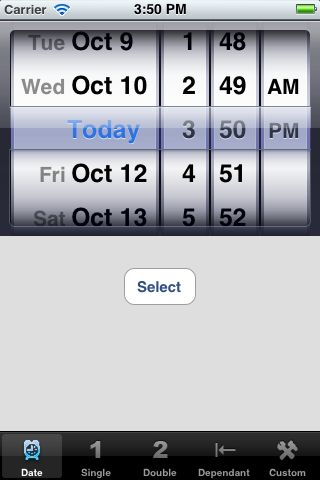
\includegraphics[width=4cm]{1.jpg} %ou image.png, .jpeg etc.
\caption{Date Picker} %la légende
\label{api} %l'étiquette pour faire référence à cette image
\end{figure} %on ferme l'environnement figure 
 
\begin{figure}[!h] %on ouvre l'environnement figure
\centering
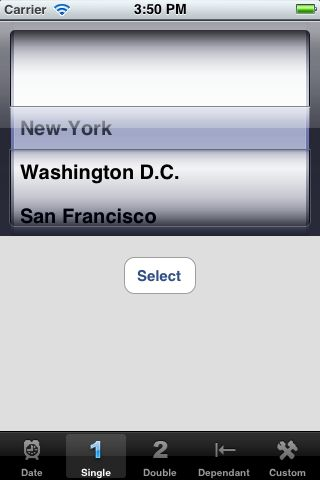
\includegraphics[width=5cm]{2.jpg} %ou image.png, .jpeg etc.
\caption{Single Picker} %la légende
\label{api} %l'étiquette pour faire référence à cette image
\end{figure} %on ferme l'environnement figure

 
\begin{figure}[!h] %on ouvre l'environnement figure
\centering
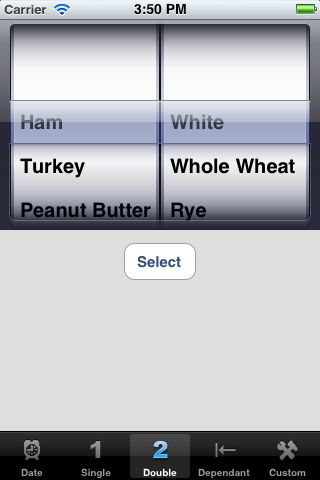
\includegraphics[width=5cm]{3.jpg} %ou image.png, .jpeg etc.
\caption{Double Picker} %la légende
\label{api} %l'étiquette pour faire référence à cette image
\end{figure} %on ferme l'environnement figure
 

\begin{figure}[!h] %on ouvre l'environnement figure
\centering
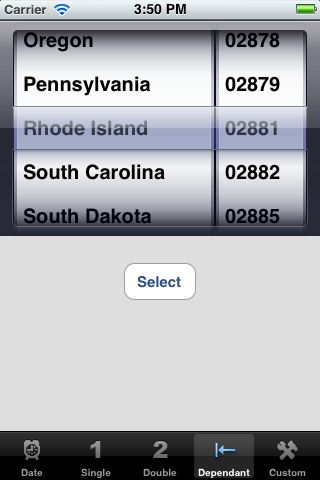
\includegraphics[width=5cm]{4.jpg} %ou image.png, .jpeg etc.
\caption{Dependant Picker (ZIP codes associated with the State)} %la légende
\label{api} %l'étiquette pour faire référence à cette image
\end{figure} %on ferme l'environnement figure
 

\begin{figure}[!h] %on ouvre l'environnement figure
\centering
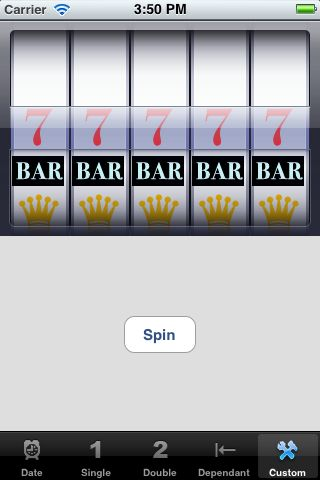
\includegraphics[width=5cm]{5.jpg} %ou image.png, .jpeg etc.
\caption{First view of the Slot Machine} %la légende
\label{api} %l'étiquette pour faire référence à cette image
\end{figure} %on ferme l'environnement figure


\begin{figure}[!h] %on ouvre l'environnement figure
\centering
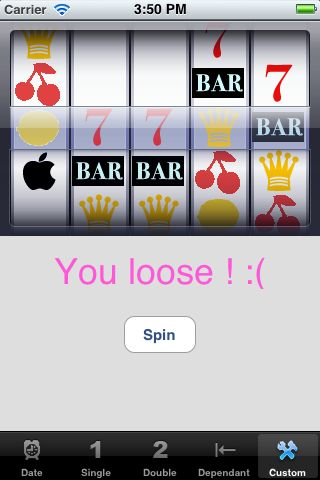
\includegraphics[width=5cm]{6.jpg} %ou image.png, .jpeg etc.
\caption{Second view of a loosing game - slot machine } %la légende
\label{api} %l'étiquette pour faire référence à cette image
\end{figure} %on ferme l'environnement figure


\begin{figure}[!h] %on ouvre l'environnement figure
\centering
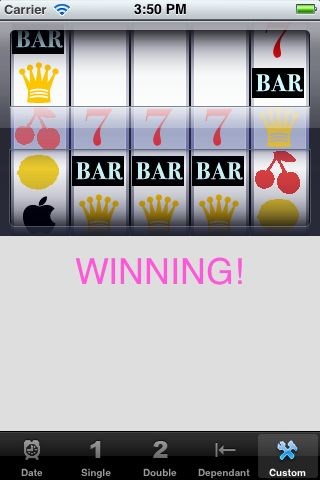
\includegraphics[width=5cm]{7.jpg} %ou image.png, .jpeg etc.
\caption{Third view of a winning game - slot machine} %la légende
\label{api} %l'étiquette pour faire référence à cette image
\end{figure} %on ferme l'environnement figure

 
\end{document}

